\chapter{Introdução}

\section{Motivação}

O uso de Veículos Autônomos Aéreos Não Tripulados (VAANTs), também conhecidos como \textit{drones} ou quadrotores autônomos, vêm ganhando notoriedade nas últimas décadas devido à sua alta versatilidade, manobrabilidade, avanço tecnológico computacional, seguido também de aplicações inovadoras em quase todos os setores, sejam elas com propósito militar, de pesquisa, comércio, vigilância ou de lazer. Justifica-se também este interesse por conta do crescente número de fabricantes, redução de preços, melhoria da qualidade dos componentes e sensores envolvidos, demandando assim técnicas mais robustas para garantir a segurança das aeronaves \cite{Santos2014}.

Segundo definições de \citet{Duan2010}, VAANT é um tipo de sistema muito complexo que integra diferentes componentes de hardware, como o Sistema de Posicionamento Global (GPS), Unidade de Gerenciamento Inercial (IMU), controlador e diferentes componentes de software, como processamento de imagem e planejamento de trajetória. \citet{Costa2012} destaca a importância da IMU no sistema de localização dos VAANTs que integra bússola, barômetro, sonares e sensor GPS. Tanto o IMU quanto a bússola indicam a atitude; Barômetro e sonar podem ser usados para leitura de altitude, e o GPS para obter dados de posicionamento e também altitude. 

\subsection{Problematização da Descolagem e Pouso}

Contudo, estes sensores de navegação podem apresentar erros da ordem de metros e de forma acumulativa, principalmente quando se diz a respeito de pousos ou decolagens utilizando GPS próximos a prédios, redes elétricas ou montanhas que bloqueiam ou anulam completamente o sinal de GPS. Este fato deprecia a qualidade, confiabilidade e custo da missão, visto que se faz necessário a aquisição de sensores com altíssima precisão e com blindagem eletrostática específica, resultando em custo elevado. Logo, a visão computacional é uma excelente solução de baixo custo e alto retorno de informações espaciais para o controle de VAANTs.
 
Tal solução é apresentada através das câmeras de sensor exteroceptivo ou monocular, que além de atribuir precisão em navegação possui a vantagem de ser um sensor passivo, de baixa sensibilidade a ruídos e independente do sinal de GPS, permitindo voo em ambientes onde esse sinal não possui boa qualidade \cite{GUO2014}. Pode-se citar algorítimos de código aberto como de \citet{Forster2014} e \citet{Raul2016}, que trazem robustas soluções de navegação por visual monocular através de uma abordagem semi-direta que elimina a necessidade de extração de recursos caros e técnicas de correspondência robustas para estimativa de posição e orientação.

%===================================================================================================

\subsection{Aplicação de Drones em Serviçoes de encomendas \textit{(delivery)}}

Uma das aplicações dos estudos desta tecnologia está presente no setor de encomendas \textit{(delivery)}, onde são utilizados pelo serviço de entregas em algumas regiões como nos Estados Unidos, Austrália e Suíça. Um dos exemplos é o serviço \textit{Prime Air} da companhia \textit{Amazon}, que promete atender a encomendas de até 5 \textit{libras} em meia hora, com veículos cobertos de redundâncias "\textit{sense and avoid}" para garantir a segurança durante o tráfego em rotas especiais. Na Suíça estão sendo testados \textit{drones} para entregas de encomendas pesando até um quilograma por distâncias que se estendem a dez quilômetros, segundo notícias de Agosto de 2016 \cite{Vidal2016}.

Segundo notícias de Maio de 2018. O Brasil já realizou a primeira simulação de \textit{delivery}, que ocorreu em São Paulo com autorização do Departamento de Controle do Espaço Aéreo (DECEA). Com o objetivo de entregar medicamentos, a ação utilizou um hexacóptero e um programa desenvolvidos pela marca nacional \textit{SMX Systems}. Apesar de ser considerada a primeira simulação oficial, esta não foi a primeira vez em que uma entrega é feita com \textit{drone} no país, já que em 2014 houve um \textit{delivery} de pizza no município de Santo André (SP) \cite{Techtudo2018}.


\subsection{Problematização Linhas de Transmissão}

Segundo \citet{Gilberto2016} Uma das principais limitações dos VAANTs em praticamente todos os tipos de aplicações é a carga útil limitada que eles podem carregar. Esta situação limita a quantidade de baterias transportadas durante uma missão que, consequentemente, restringe o tempo de voo. Devido a essa limitação, os veículos voadores precisam retornar a uma estação de recarga após um curto período de operação. Neste contexto, a aterrissagem autônoma torna-se essencial para economizar energia em missões do tipo \textit{perch-and-stare} em que a manutenção do voo não é necessariamente necessária. Além disso, ao realizar tarefas em que seja necessário um voo longo contínuo ou viagens de longa distância, o retorno a uma estação base não é prático. Nesses cenários, seria mais conveniente implantar uma estação base móvel capaz de transportar energia suficiente para vários ciclos de recarga. Os VAANTs, então, teriam que realizar pouso periódico autônomo em estações de ancoragem baseadas em terra ou voadoras para recarregar e se tornar operacional novamente.

\subsection{Sugestão da Solução}

Com base nos argumentos descritos acima, verifica-se a motivação da tesa no âmbito de desenvolver e simular um sistema para VAANT do tipo quadrotor capaz de aterrissar de forma autônoma um alvo pré-definido e estático. A tese visa realizar o controle do VAANT usando apenas sensoriamento por visão e computação embarcada, sem depender de qualquer infraestrutura externa. A simulação é feita via V-REP usando linguagem \textit{Python} e captura de imagem monocular. O algorítimo inicialmente detecta o local de decolagem/pouso via marcador fiducial \textit{tag} \textit{ArUco}, em seguida retorna a posição do quadrotor em relação ao marcador, contornando erros inerentes a sensores de posicionamento, como IMU e GPS. O diferencial da proposta baseia-se em obter um algorítimo que utilize a Rede Neural Convolucional (CNN) de forma a complementar a detecção da \textit{tag} \textit{ArUco} clássica da maneira mais eficaz. Deseja-se criar dados de treinamento híbridos através de dados sintéticos e reais de forma a superar a limitações de casos específicos como detecção imprecisa a longa distância, oclusão parcial ou uso de câmeras com alta distorção. 

Verifica-se a utilização de \textit{ArUco} pelo fato de ser uma biblioteca de código aberto para detecção de marcadores fiduciais. Segundo \citet{Aruco2014}, a biblioteca permite estimar a pose de uma câmera a partir de um ou vários marcadores que são analisados em paralelo, onde, cria-se uma imagem canônica no nível da pirâmide que alcança o melhor equilíbrio entre qualidade e tamanho, sendo atualmente uma das estratégias mais investigas para uso como marcador de pouso e rastreamento com VAANTs, além de dispor de criação de marcadores personalizados. 

%Contudo, tem-se ainda o desafio de identificação a longo alcance, visto que o marcador fiducial tem um limite de tamanho por distancia de identificação segura. Ou seja, para alturas elevadas acima de 30 metros se faz necessário o uso de uma segunda abordagem, um algoritmo de odometria visual monocular que mesmo sem a identificação do marcador, guie o \textit{drone} próximo a altura de identificação segura. 

%===================================================================================================

%Logo o trabalho traz a proposta de se utilizar a biblioteca ArUco  em conjunto com o algorítimo de \citet{Forster2014}, uma técnica já consolidada e precisa que segundo o autor a mais rápida dos métodos atuais de última geração. Tem-se como vantagem, a abordagem semi-direta que elimina a necessidade de extração de recursos caros e técnicas de correspondência robustas para estimativa de movimento. O algorítimo opera diretamente nas intensidades de pixel, o que resulta em precisão de subpixel em altas taxas de quadros. Chamado pelo autor como abordagem de \textit{Odometria Visual Semi-Direta} (SVO), já foi testado em veículos micro-aéreos e lançado como \textit{software} de código aberto.

%Em relação ao desafio de custo elevado versos desempenho computacional, conta-se com a estratégia de embarcar o \textit{software} desenvolvido em um \textit{hardware} de dispositivo \textit{smartphones} via plataforma \textit{Android} com o objetivo obter desempenho computacional bom ou similar a computadores convencionais quando utilizados para o mesmo objetivo. As vantagens de se embarcar uma interface \textit{Android} é facilidade de comunicação e uso dos periféricos já embarcados no dispositivo, além dos ganhos em custo benefício entre processamento e consumo de energia.

%Por fim, serão realizados testes experimentais que verifiquem o desempenho do sistema desenvolvido frente a 2 (duas) abordagens utilizadas para pouso de precisão: 1.PX4Flow via técnica Optical Flow; 2.IR-LOCK via câmera PIXY. Estima-se o uso do sistema em uma aplicação real em missões de entregas (\textit{deliveries}) de medicamento na cidade do Porto-Portugal vinculada a empresa \textit{Connec Robotics}. As mesmas técnicas utilizadas para o pouso bodem ser replicadas para a decolagem que também apresenta grandes problemáticas quando guiada somente por GPS. 

%\subsection{Objetivo}

%O presente trabalho tem como objetivo principal desenvolver e simular um sistema de decolagem e pouso de precisão autônoma para um VAANT do tipo quadrotor. A tese visa realizar o controle do sistema utilizando somente técnicas de visão computacional simuladas via V-REP usando um quadrotor com câmera monocular. O algorítimo inicialmente detecta o local de decolagem/pouso via marcador fiducial \textit{tag} ArUco, em seguida retorna a posição do quadrotor em relação ao marcador, contornando erros inerentes a sensores de posicionamento, como IMU e GPS. O diferencial da proposta baseia-se em obter um algorítimo que utilize a Rede Neural Convolucional (CNN) de forma a complementar a detecção da \textit{tag} ArUco clássica da maneira mais eficaz. Deseja-se criar dados de treinamento híbridos através de dados sintéticos e reais de forma a superar a limitações de casos específicos como detecção imprecisa a longa distância, oclusão parcial ou uso de câmeras com alta distorção.

    \vspace{\fill}

%\begin{itemize}
    
    %A metodologia adotada demanda as seguintes etapas:
    
  %\item Realizar levantamento bibliográfico sobre os principais conceitos e desafios de pesquisa referentes a pouso e decolagem de precisão autônoma utilizando veículos quadrotores;
  
  %\item Embarcar bibliotecas de OpenCV, ArUco e \textit{Tensorflow}  vinculados a linguagem de programação C/C++ ou \textit{Python} em uma única IDE;
  
  %\item Estruturar um dicionário de marcadores fiduciais que apresente bons desempenhos nos quesitos de identificação precisa do marcador e confiabilidade de posição;
  
  %\item Desenvolver inicialmente um algorítimo que tenha como saída a posição do marcador de pouso em relação ao quadrotor, baseada somente na técnica de detecção via \textit{tag} ArUco;
  
  %\item Utilizar o Simulador V-REP para integrar a comunicação de controle do quadrotor com o algorítimo desenvolvido;
  
   %\item Realizar a aquisição de dados sintéticos de treinamento de rede neural através de ensaios simulados de decolagem e pouso com quadrotores via V-REP;
  
  %\item Realizar a aquisição de dados reais de treinamento de rede neural através de ensaios reais de decolagem e pouso com quadrotores via gravações de \textit{datasets};
   
   %\item  Realizar treinamento dos dados obtidos para identificar o marcador desejado utilizando técnica de Rede Neural Convolucional (CNN);
   
   %\item Implementar e simular no V-REP o algorítimo desenvolvido (CNN) de forma a complementar a detecção da \textit{tag} ArUco clássica da maneira mais eficaz.
   
   %\item Coletar dados estatísticos dos ensaios simulados via V-REP e analisar o desempenho do sistema autônomo projetado;
   
    %\item Determinar os melhores parâmetros visando eficiência na identificação de marcadores a longa distância, onclusões parciais e distorção de câmera;
    
%\end{itemize}

%===================================================================================================

\section{Estado da Arte}

%\subsection{Visão Geral: Veículos Autônomos Aéreos Não Tripulados VAANTS}

	%\subsubsection{Conceitos e Fundamentos}

	%\subsubsection{Desafios de Controle e Navegação em Pouso/Decolagem}

	%\subsubsection{Aplicações Comerciais}

%\subsection{Trabalhos Relacionado: Descolagem e Pouso Autônomo}

	%\textbf{Revisão Literária das Principais Técnicas de Decolagem e Pouso}

	%\textbf{Revisão Literária do Uso de Marcadores Fiduciais como \textit{Landmarks}}

	%\textbf{Revisão Literária das Técnicas de Redes Neurais Usadas para Aperfeiçoar a Detecção de \textit{Tags} ArUco}
	
	Neste tópico, será abordado uma revisão literária sobre as principais técnicas utilizadas para decolagem e pouso de precisão para VAANT do tipo quadrotor, bem como, a revisão literária do uso de marcadores fiduciais, abordando os principais trabalhos que utilizam técnicas para detecção de marcadores visuais como solução do problema de localização. Priorizou-se técnicas que utilizaram somente visão computacional a fim de criar um estado da arte mais próximo do proposta pela tese, a qual visa contornar erros inerentes a sensores de posicionamento como IMU e GPS ou sensores ativos como lasers e sonares. 
	
	\subsection{Revisão Literária das Principais Técnicas de Decolagem e Pouso}
	
	Inciailmente é realizada uma revisão literária das principais técnicas de decolagem e pouso, a qual é exposta de forma resumida através da Tabela~\ref{qd:estado-da-arte}, onde, destaca-se a principal abordagem e contribuição científica de cada referência. Em seguida, realiza-se uma análise comparativa destes trabalhos em relação ao trabalho proposto e os principais desafios superados por cada técnica, sendo o principal objetivo deste tópico. 
	
    \begin{table}[H]
    \centering
	\caption{Resumo das principais abordagens e contribuições científicas relacionadas à decolagem e pouso de VANTs usando somente visão computacional.}
	%\vspace{0.5cm}
	\begin{tabular}{ccc}
		   
	\hline
	\multirow{2}{*}{\textbf{Abordagem}} & \multirow{2}{*}{\textbf{Contribuição}} & \multirow{2}{*}{\textbf{Referências}} \\
	\\ \hline
	\multirow{3}{*}{Odometria Monocular}  & \multirow{3}{*}{Sistema de Pouso Autônomo} &  \\
	\multirow{3}{*}{Estimação da Plataforma} &  \multirow{3}{*}{em Plataforma Móvel}  & \multirow{2}{*}{\citet{Falanga2017}} \\
	&                                  &                         &                       \\ \hline
	\multirow{3}{*}{Modelo de Controle}  & \multirow{3}{*}{Geração de Trajetória de Pouso} &  \\
	\multirow{3}{*}{Preditivo (MPC)} &  \multirow{3}{*}{e Robustez do Controlador}  & \multirow{2}{*}{\citet{Gilberto2016}} \\
	&                                  &                         &                       \\ \hline
	\multirow{3}{*}{Marcador QR-Code}  & \multirow{3}{*}{Pouso Autônomo Preciso} &  \\
	\multirow{3}{*}{GPS + Navegação Ótica} &  \multirow{3}{*}{em Relação ao GPS Isolado}  & \multirow{2}{*}{\citet{Maiman2017}} \\
	&                                  &                         &                       \\ \hline
	\multirow{3}{*}{Visão Computacional}  & \multirow{3}{*}{Pouso Autônomo} &  \\
	\multirow{3}{*}{Operações Morfológicas} &  \multirow{3}{*}{Somente Técnicas de Visão}  & \multirow{2}{*}{\citet{Vidal2016}} \\
	&                                  &                         &                       \\ \hline
	\multirow{3}{*}{Orientação de Navegação}  & \multirow{3}{*}{Geração de Trajetórias de Pouso} &  \\
	\multirow{3}{*}{Intrínseca de Tau} &  \multirow{3}{*}{ Baseado Espaço-Temporal em 4D}  & \multirow{2}{*}{\citet{Vetrella2017}} \\
	&                                  &                         &                       \\ \hline
	\end{tabular}

	\label{qd:estado-da-arte}
\end{table}

    A literatura sugere que a maioria das implementações de técnicas para decolagem e pouso disponíveis podem ser classificadas em 2 (duas) categorias: A primeira com sistemas que fazem uso de sensores de imagem e a segunda com sistemas cujas capacidades de navegação são baseadas em sensores ativos, como lasers, sonares em casos de ambientes internos e IMU e GPS em casos de ambiente externo.
    
    Destaca-se inicialmente o trabalho de \citet{Falanga2017}, que traz uma abordagem prática, contando com um algorítimo de visão computacional avançado, fusão de multi-sensores para localização do veículo aéreo além de detecção e estimativa de movimento da plataforma móvel usando uma segunda câmera. O algorítimo de detecção visual da plataforma móvel é aplicado em um filtro de \textit{Kalman} atrelado ao modelo cinemático da plataforma, resultando em uma identificação da plataforma móvel com alta frequência.
    
    O principal diferencial entre o trabalho de \citet{Falanga2017} e a tese apresentada é em relação a estratégia de detecção do marcador visual, que não utiliza redes neurais convolucionais. A principal contribuição do trabalho de \citet{Falanga2017} são os resultados práticos do pouso autônomo, que diferente da proposta da presente tesa, visa um pouso em uma plataforma móvel, tendo como maior diferencial a utilização de um rápido algorítimo de odometria monocular de \cite{Forster2014}. Figura~\ref{fig:estadolanding}.
    
    %  Figura.
    \begin{figure}[H]
    	\centering
    	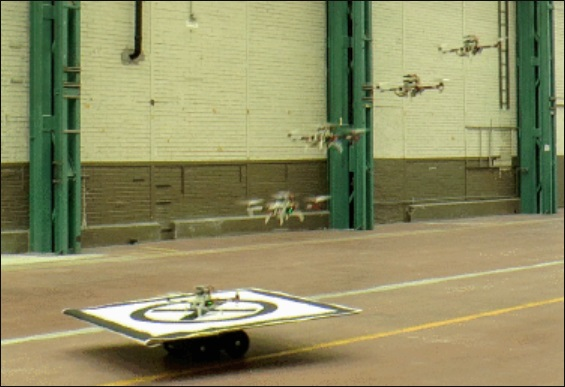
\includegraphics[scale=1.1]{figuras/landing.jpg}
    	\caption{Quadrotor pousando em uma plataforma móvel,~\cite{Falanga2017}.}
    	\label{fig:estadolanding}
    \end{figure}
    
    Outro trabalho de relevância é o de \citet{Gilberto2016}, que também tem como objetivo a realização prática de pouso em plataforma móvel, contudo, utilizando micro-veículos aéreos (MAVs). Verifica-se também uma abordagem diferente do proposto pela presente tese, a qual é voltada ao desenvolvimento de um algorítimo de controle através do Modelo de Controle Preditivo (MPC). Esta abordagem considera o problema da robustez de uma forma viável do ponto de vista da implementação do sistema, tendo como principal contribuição científica a geração de uma trajetória ótima, projetada para melhorar o desempenho do controlador e garantir robustez no sistema.
    
    Ainda referente a trabalhos com pouso autônomo, destaca-se o trabalho de \citet{Maiman2017}, que cria uma nova solução precisa e econômica para pouso com \textit{drones}. Diferente do objetivo proposto pela presente tese, o algorítimo desenvolvido por \citet{Maiman2017} chamado de \textit{GOLD} combina GPS com navegação ótica para reconhecer e descer de forma iterativa em direção a um ponto de pouso alvo o qual é identificado via detecção QR-Code. O trabalho traz como contribuição científica um pouso autônomo de baixo custo e mais preciso do que um sistema que utilize somente GPS.
    
    Verifica-se o trabalho de \citet{Vidal2016} relevante para identificar os conceitos essenciais de um sistema de pouso autônomo que utiliza somente técnicas de visão computacional. O trabalho traz uma abordagem de visão computacional pura, utilizando somente técnicas de obtenção de contorno e reconhecimento de formas por operações morfológicas, \textit{thresholding} e outras técnicas matemáticas a fim de se obter processamento rápido e simples. O diferencial entre o trabalho de \citet{Vidal2016} e a tese apresentada é a técnica de detecção visual do marcador que não utiliza marcadores fiducial do tipo \textit{Tag} como \textit{ArUco}, \textit{AprilTag}, \textit{ARToolkit}, \textit{ARTag} ou \textit{QR-Code} e nem detecção avançada por rede neural. Tendo como contribuição científica a validação e implementação de técnicas simples e de rápido processamento em visão computacional, voltada para identificação de contorno e reconhecimento de forma por morfologia para pouso de \textit{drones} autônomos.
    
    No trabalho de \citet{Vetrella2017}, desenvolveu-se um algoritmos flexível de geração de trajetória, sua contribuição científica permitiu altos níveis de autonomia para as fases críticas da missão, como decolagem, cobertura de área e pouso. Diferente da tesa apresentada, o trabalho de \citet{Vetrella2017} apresenta uma abordagem de orientação que usa a teoria de orientação intrínseca da \textit{Tau} aprimorada para criar trajetórias espaço-temporais em 4D para um tempo-para-contato desejado com uma plataforma de aterrissagem rastreada por um sensor visual.
    
%====================================================================

    \subsection{Revisão Literária do Uso de Marcadores Fiduciais como \textit{Landmarks}}
    
    A seguir, realiza-se uma revisão literária sobre o uso de marcadores fiducuais como marcadores de localização (\textit{Landmarks}),  abordando os principais trabalhos que utilizam técnicas para detecção de marcadores visuais como solução do problema de localização.
    
    A principal motivação de usar sensores de imagem é seu peso leve e baixo consumo de energia. Para este fim, a literatura sugere várias abordagens que utilizam marcadores visuais para simplificar a problema de localização, como exemplo, têm-se o trabalho de \citet{Pestana2016}, que faz uso de marcadores visuais \textit{ArUco} \citet{Salinas2013}, a abordagem proposta por \citet{Jayatilleke2013} que requer um conhecimento prévio de todas as poses de referência, enquanto que em \citet{Faigl2013}, o VAANT é necessário para manter os marcadores externos sempre visíveis. Nessas abordagens, o uso de marcadores visuais fornece uma localização precisa, com a desvantagem de alterar a área a ser explorada.
    
    Marcadores planares quadrados tornaram-se um método popular para estimar poses em aplicações como robôs autônomos \citet{Robert2009}, \citet{Pichler2017} e \citet{Valencia2005}, veículos não tripulados, \citet{Broggi2000}, \citet{Patterson2014} e \citet{Gonzalez2017}, além de treinadores virtuais \citet{Pflugi2017}, \citet{Chen2016} e \citet{Khattak2014}. Os marcadores permitem estimar a posição de uma câmera monocular com custo mínimo, alta robustez e velocidade. Basta criar marcadores com uma impressora normal, colocá-los no ambiente desejado para cobrir a área de trabalho e registrar sua localização a partir de um conjunto de imagens.
    
    Existem vários tipos de marcadores, cada um deles pertencente a um dicionário. Cada biblioteca propôs seu próprio conjunto de marcadores. Então, temos \textit{ArToolKit+}, \textit{Chilitags}, \textit{AprilTags} e, claro, o dicionário \textit{ArUco}. O \textit{design} de um dicionário é importante, já que a ideia é que seus marcadores sejam o mais diferentes possíveis para evitar confusões. 

    Um sistema de referência fiducial é composto por um conjunto de marcadores válidos e um algoritmo que realiza sua detecção e possivelmente correção em imagens. Vários sistemas de marcadores fiduciais têm sido propostos na literatura como mostrado na Figura ~\ref{fig:aruco-tipos}.

    %  Figura.
    \begin{figure}[H]
    	\centering
    	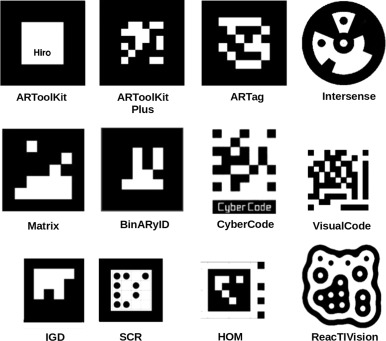
\includegraphics[width=10cm, height=8 cm]{figuras/aruco-tipos.jpg}
    	\caption{Exemplos de outros tipos de marcadores fiduciais,~\cite{Garrido2016}.}
    	\label{fig:aruco-tipos}
    \end{figure}

    As propostas mais simples consistem em usar pontos como marcadores fiduciais, como LEDs, esferas retrorreflexivas ou planas \cite{Klaus1998, Ribo2001}, que podem ser segmentadas usando técnicas básicas sob condições controladas. Sua identificação é geralmente obtida a partir da posição relativa dos marcadores e geralmente envolve um processo complexo. Outras abordagens usam marcadores circulares planares onde a identificação é codificada em setores circulares ou anéis concêntricos \cite{Measurements1998, Naimark2002}. No entanto, os marcadores circulares geralmente fornecem apenas um ponto de correspondência (o centro), tornando necessária a detecção de vários deles para estimar a pose.

    Outros tipos de marcadores fiduciais são baseados na detecção de \textit{blob}. \textit{Cybercode} \cite{Rekimoto2000} ou \textit{VisualCode} \cite{Michael2004} é derivado da tecnologia de códigos de barras 2D como \textit{MaxiCode} ou \textit{QR}, mas também pode fornecer com precisão vários pontos de correspondência. Outros marcadores fiduciais populares são os marcadores de amebas \textit{ReacTIVision} \cite{Kaltenbrunner2007}, que também são baseados na detecção de \textit{blob} e seu \textit{design} foi otimizado usando algoritmos genéticos. Alguns autores propuseram o uso de classificadores treinados para melhorar a detecção em casos de má iluminação e desfoque causado pelo movimento rápido da câmera \cite{Claus2005}.

    Uma alternativa para as abordagens anteriores são os sistemas de marcadores fiduciais baseados em quadrados. Sua principal vantagem é que a presença de quatro pontos proeminentes pode ser empregada para obter a pose, enquanto a região interna é usada para identificação (usando um código binário ou um padrão arbitrário, como uma imagem). Na categoria de padrões arbitrários, um dos sistemas mais populares é o \textit{ARToolKit} \cite{Kato1999}, um projeto de código aberto que tem sido amplamente utilizado na última década, especialmente na comunidade acadêmica. Marcadores \textit{ARToolKit} são compostos por uma borda preta larga com uma imagem interna que é armazenada em um banco de dados de padrões válidos. Apesar de sua popularidade, tem algumas desvantagens. Primeiro, ele usa uma abordagem de correspondência de modelos para identificar marcadores, obtendo altas taxas de confusão de falsos positivos e inter-marcadores \cite{Fiala2005} . Em segundo lugar, o sistema usa um limiar global fixo para detectar quadrados, tornando-o muito sensível a diferentes condições de iluminação.
    
    Outras abordagens baseadas em sensores de imagem para realizar a navegação e localização, evitar colisões são os trabalhos de \citet{Zingg2010} e \citet{Lippiello2011}, onde \textit{Pyramidal Lukas-Kanade} é usado para a estimativa do fluxo óptico. As técnicas utilizam informações computadas por algoritmos de fluxo óptico para obter um mapa de profundidade.
    
    Outras abordagens interessantes e mais inovadoras usam o Redes Neurais para classificação e navegação de cenas internas \citet{Kim2015}, utilizando uma \textit{Convolutional Neural Network} (CNN) para aprender uma estratégia de controle baseada em dados capturados de vôos realizados por um piloto especialista humano.
    
    APRESENTAR AQUI UM RESUMO DAS ATIVIDADES DO GRUPO  DE AUTOMACAO E ROBOTICA DO LABORAT'ORIO DE PROCESSAMENTO DE SINAIS E AN'ALISE DE SISTEMAS DINAMICOS DO DS1 DA FEM, E COMO ESSE TRABALHO SE INSERE NOS OBJETIVOS DESSE GRUPO
    
    APRESENTAR AQUI TAMBEM UMA INDICACAO DAS PUBLICA'COES E OUTRAS ATIVIDADES DE VALOR REALIZADAS DURNTE O PER'IODO DO DOUTORADO
    
    %abordagem que utiliza marcadores fiduciais clássicos ...abordagem que utiliza PX4Flow via técnica Optical Flow e IR-LOCK via câmera PIXY. 
    

%===================================================================================================

\section{Contribuição Científica}
    
    Na presente tese, apresenta-se um sistema validado por simulação via V-REP para VAANT do tipo quadrotor capaz de decolar e pousar de forma autônoma em um alvo estático. O algorítimo é baseado somente em técnicas de visão computacional para detectar a plataforma de pouso através de marcador fiducial e assim retornar a posição do quadrotor em relação ao marcador que foi desenvolvido para ter identificação única. Logo, não há necessidade de nenhum conhecimento prévio sobre a localização da plataforma de pouso. O sistema apresenta baixo custo por eliminar a necessidade de instalação de infraestrutura externa, como um sistema de captura de movimento, além de contornar erros inerentes a sensores de posicionamento, como IMU e GPS. O algorítimo utiliza Rede Neural Convolucional (CNN) de forma a complementar a detecção da \textit{tag} \textit{ArUco} clássica da maneira mais eficaz e supera as limitações da detecção imprecisa a longa distância, oclusão parcial ou uso de câmeras com alta distorção.
    
    FALTOU FALAR DE FORMA MAIS CLARA SOBRE:
    1 - Formulação d problema de pesquisa a ser resolvido
    2 - Itemização dos pricnipais objrtivos desse trbalho
    3 - Explicitar de forma bem clara qual a sua contribuição e resultados relevantes de sua pesquisa

	%\subsection{Dicionário de Marcadores para Pouso/Decolagem de Identificação Única}

	%\subsection{Utilização da (CNN) para Complementar a detecção da \textit{tag} ArUco de forma Eficaz}

	%\subsection{Desenvolvimento de um Sistema de Baixo Custo para Decolagem e Pouso Autônomo de Quadrotores sem uso de GPS ou IMU}

\section{Estruturação da Tese}

Os capítulos seguintes descrevem o trabalho da seguinte forma: O capítulo 2 (dois) apresenta o marcador fiducial utilizado como plataforma de pouso, descrevendo seus principais conceitos; O capítulo 3 (três) aborda sobre a técnica de rede neural utilizadas complementarmente na detecção da plataforma de pouso; O capítulo 4 (quatro) descreve o ambiente de simulação, expondo a plataforma usada e as características do veículo aéreo e controlador utilizado; O capítulo 5 (cinco) define as tarefas realizadas e apresenta os resultados e discussões; Por fim, o capítulo 6 (seis) aborda todas as conclusões do trabalho realizado e sugestões de trabalhos futuros.




